\documentclass[10pt,twocolumn]{article}
\usepackage{amsmath,graphicx,fullpage,booktabs,microtype}
\usepackage[font={sc,footnotesize}]{caption,subfig}
\bibliographystyle{abbrv}

\newcommand{\degree}{\ensuremath{^\circ}}
\newcommand{\prfB}{\emph{prfB}}
\newcommand{\rpoS}{\emph{rpoS}}
\heavyrulewidth=.125em
\thispagestyle{empty}
\begin{document}

\title{{\bf \rpoS}}
\author{{\sc H. Lian, V. Bhattcharya, and D.R. Vitek}}
\date{{\sc \today}}
\maketitle

\section{Analyzing \rpoS}

The RNA polymerase sigma factor \rpoS\ is known to be translationally regulated.
This report aims to analyze potential areas of the sequence where transcriptional regulation can occur.
It also suggests changes to the sequence that may improve yield for \rpoS\.

\subsection{Polar Plot}

The polar plot for \rpoS\ (Figure~\ref{rpos:polar}) is similar to those for other normal genes; 
it remains near the species angle.

\begin{figure}[htp]
    \centering
    \caption{Original \rpoS\ Sequence}
    \label{rpos:polar}
    {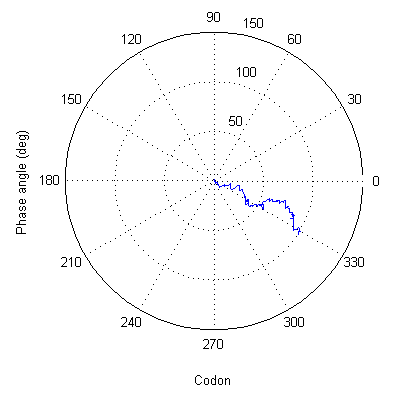
\includegraphics[scale=0.7]{rpoS_polar.png}}
\end{figure}

\subsection{Displacement Plots}

Unexpectedly, the displacement plot for \rpoS\ (Figure~\ref{rpos:disp}) does not show any interesting behavior.
The displacement stays within the range $[-0.5,0.5]$, which is well outside the trouble region of $-1$ or 1.

\begin{figure}[htp]
    \centering
    \caption{Original \rpoS\ Displacement Plot}
    \label{rpos:disp}
    {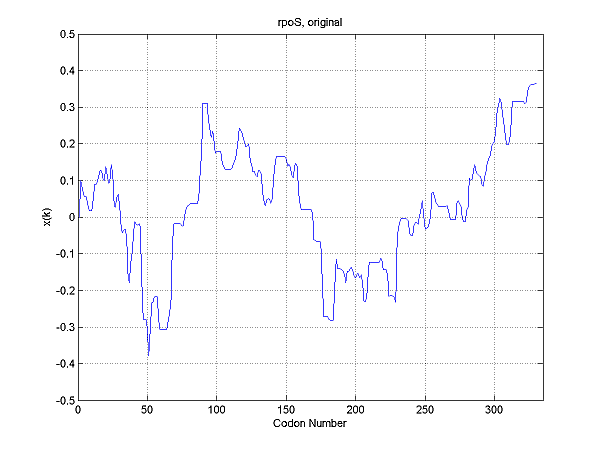
\includegraphics[scale=0.8]{rpoS.png}}
\end{figure}

On a more sensitive model, however, \rpoS\ shows a different displacement plot.  
Figure~\ref{rpos:sensdisp} graphs ten iterations of \rpoS\ on the sensitive model.

\begin{figure}[htp]
    \centering
    \caption{Original \rpoS\ on a Sensitive Model}
    \label{rpos:sensdisp}
    {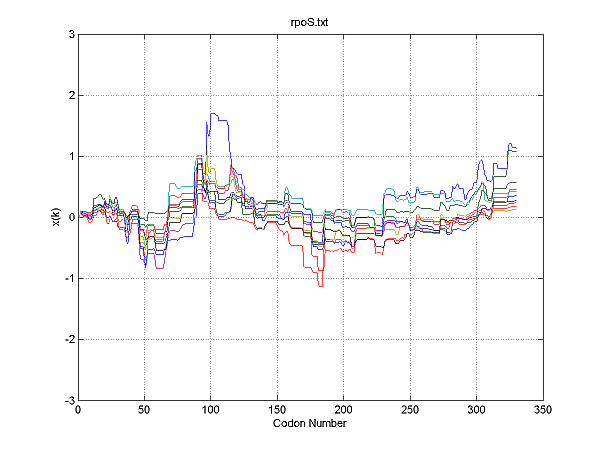
\includegraphics[scale=0.8]{rpoS_sens.png}}
\end{figure}

Figure~\ref{rpos:sensdisp} indicates that \rpoS\ has two areas where frameshifts may potentially occur.
The first such point occurs at approximately codon 95, when the displacement plot nears 1.
In fact, one iteration actually exceeds 1.5 in displacement.
Another point of interest exists at approximately codon 180; displacement dips close to $-1$ at this point.

\section{A Non-Frameshifting Sequence}

A brute-force algorithm was used to substitute synonymous codons in the \rpoS\ sequence to minimize the number of ``frameshifts."
The sensitive model was used as verificaiton.  A total of 33 codon changes were made.

\subsection{Displacement and Polar Plots}

On the less sensitive model, a displacement plot for the improved \rpoS\ sequence (Figure~\ref{rposmax:disp}) shows less variation than the original \rpoS\ sequence (Figure~\ref{rpos:disp}).
The more sensitive model highlights this difference even more (Figure~\ref{rposmax:sensdisp} versus Figure~\ref{rpos:sensdisp}).

\begin{figure}[htp]
    \centering
    \caption{Modified \rpoS Displacement Plot}
    \label{rposmax:disp}
    {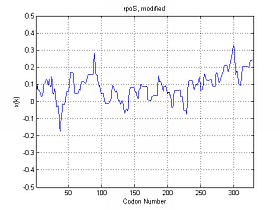
\includegraphics[scale=1]{rpoSmax.png}}
\end{figure}

\begin{figure}[htp]
    \centering
    \caption{Modified \rpoS\ on a Sensitive Model}
    \label{rposmax:sensdisp}
    {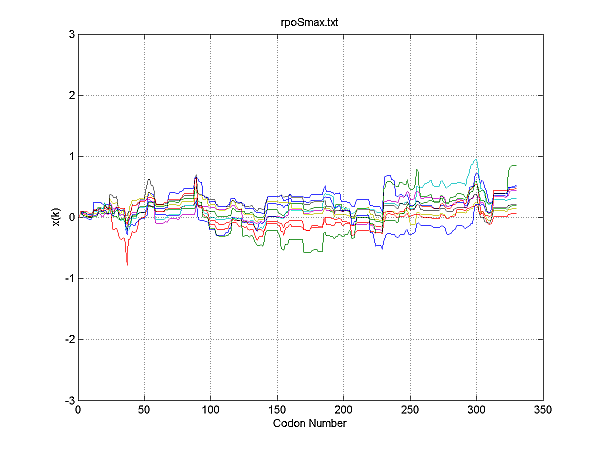
\includegraphics[scale=0.8]{rpoSmax_sens.png}}
\end{figure}

The polar plot for the modified \rpoS\ (Figure~\ref{rposmax:polar}) stays closer to the species angle as well.  
It avoids the large deviation (starting about halfway down the sequence) shown in the original polar plot (Figure~\ref{rpos:polar}).

\begin{figure}[htp]
    \centering
    \caption{Modified \rpoS\ Polar Plot}
    \label{rposmax:polar}
    {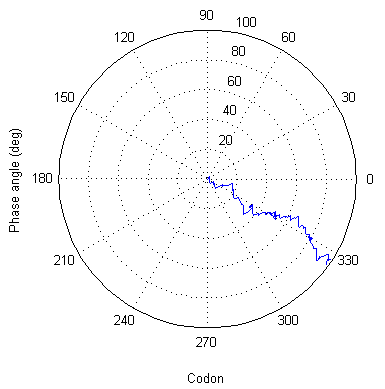
\includegraphics[scale=0.7]{rpoSmax_polar.png}}
\end{figure}

\subsection{Yields}

After 5000 iterations of the sensitive model, the original \rpoS\ sequence ran from start to finish without frameshifts 39.8\% of the time.
By contrast, the improved sequence ran properly 88.6\% of the time.

Using the sensitive model again, on 5000 iterations, the modified sequence has yield 0.2235 while the original \rpoS\ has 0.3831.

\section{A Frameshifting Sequence}

The previous section proposed a sequence to reduced deviation from the zero axis.  
The deviation was minimized with a minimum of 33 codon changes.
This section proposes a sequence with a programmed frameshift with only 3 codon changes.

\subsection{Plots}

The less sensitive model was used to draw the displacement plot because the more sensitive one always gives low yields for frameshifts (e.g., \prfB\ give 10\% yield).

Both plots are similar to those of the known frameshifter \prfB.
It is important to note the dips in the displacement plot at approximately 50 and 180 codons; the latter trouble spot corresponds to what is seen in the original sequence.
The trouble spot at codon 90 still exists (a bulge above the horizontal line $x(k)=2$), but it is not as prominent as the dip near codon 180.

\begin{figure}[htp]
    \centering
    \caption{Frameshifting \rpoS\ Displacement Plot}
    \label{rposfs:disp}
    {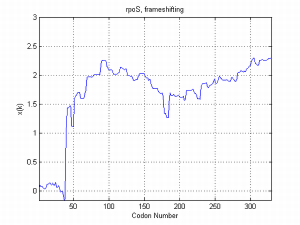
\includegraphics[scale=1]{rpoSfs.png}}
\end{figure}

\begin{figure}[htp]
    \centering
    \caption{Frameshifting \rpoS\ Polar Plot}
    \label{rposfs:polar}
    {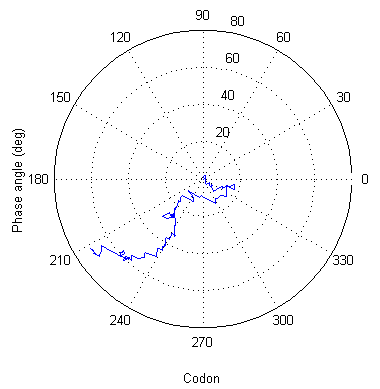
\includegraphics[scale=0.7]{rpoSfs_polar.png}}
\end{figure}

On a sample of 1000 iterations, the proper frameshift occurs 86\% of the time, but the sequence runs properly only 55.1\% of the time.

\end{document}